\subsection{Principle Component Analysis}
A Principle Component Analysis (PCA) aims at reducing the number of dimension used to represent the features of the data.
This is done by finding the eigenvectors and eigenvalues to the training set and removing some of the components representing the least variance in the data set.
Thus efficiently reducing the dimensions, but still keeping the most significant knowledge about the features.

Figure \ref{fig:contour_KvsPCA_G3M2vsRest} shows a contour plot of how well Group 3 Member 2's  handwriting was predicted successfully for $K$ and the total variance represented of the PC's varying between one and 20 and 0.5 and 1 respectively.

\begin{figure}[H]
\centering
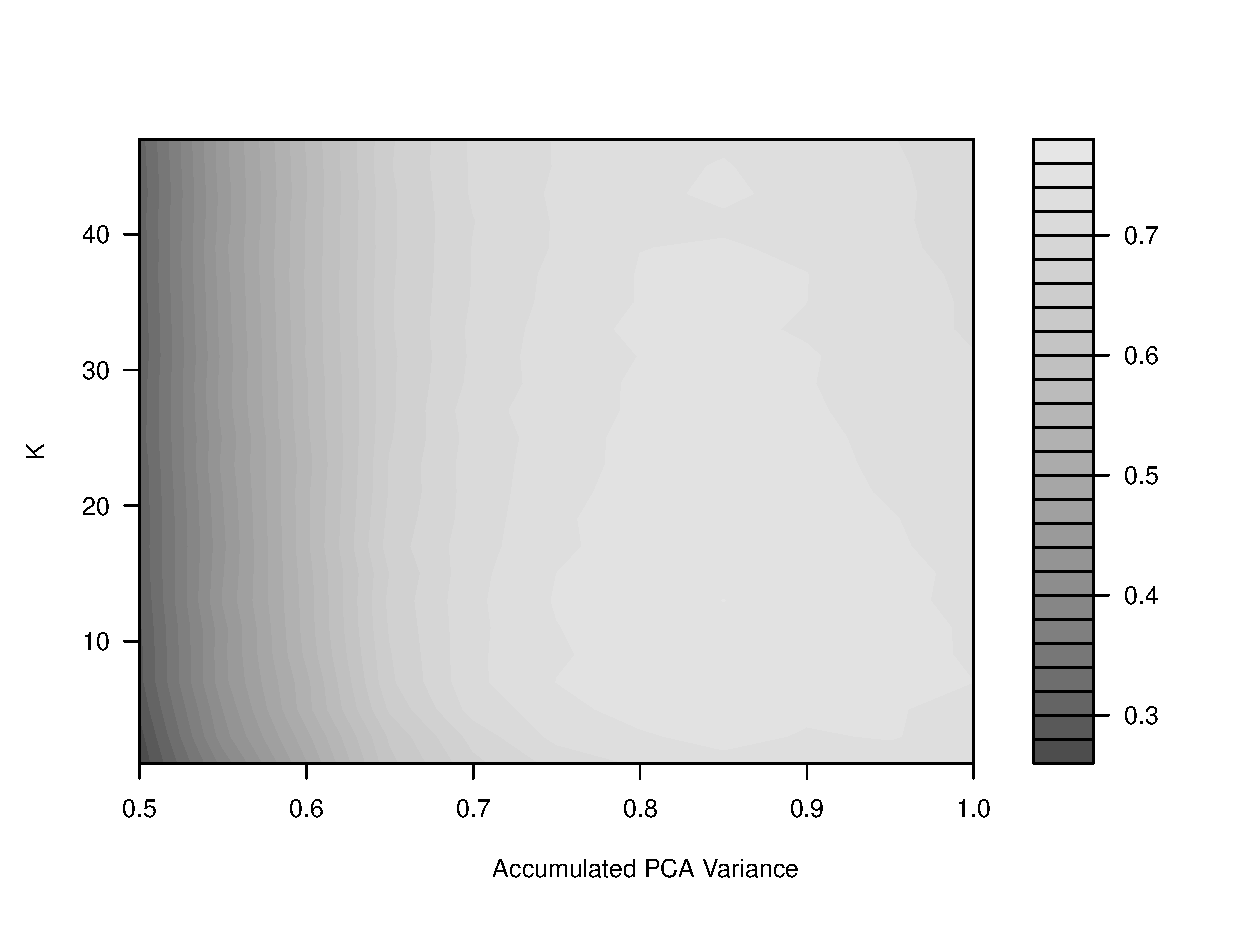
\includegraphics[width = 16cm]{graphics/contour_k_PCA_oneVsRest}
\caption{Success rate for detection of characters of Group 3 Member 2's data when he himself is not represented in the training set. 
Thewas tested with 16 people.}
\label{fig:contour_KvsPCA_G3M2vsRest}
\end{figure}


As seen on figure \ref{fig:contour_KvsPCA_G3M2vsRest}, then the optimum K and represented PCA variance is at $K = 19$ and $PCA = 0.8$. 
This is because an as high successful prediction rate is wanted, but also an as small dataset as possible. 
This point will further be used in section \ref{sec:DataNormalization}.

\begin{figure}
\centering
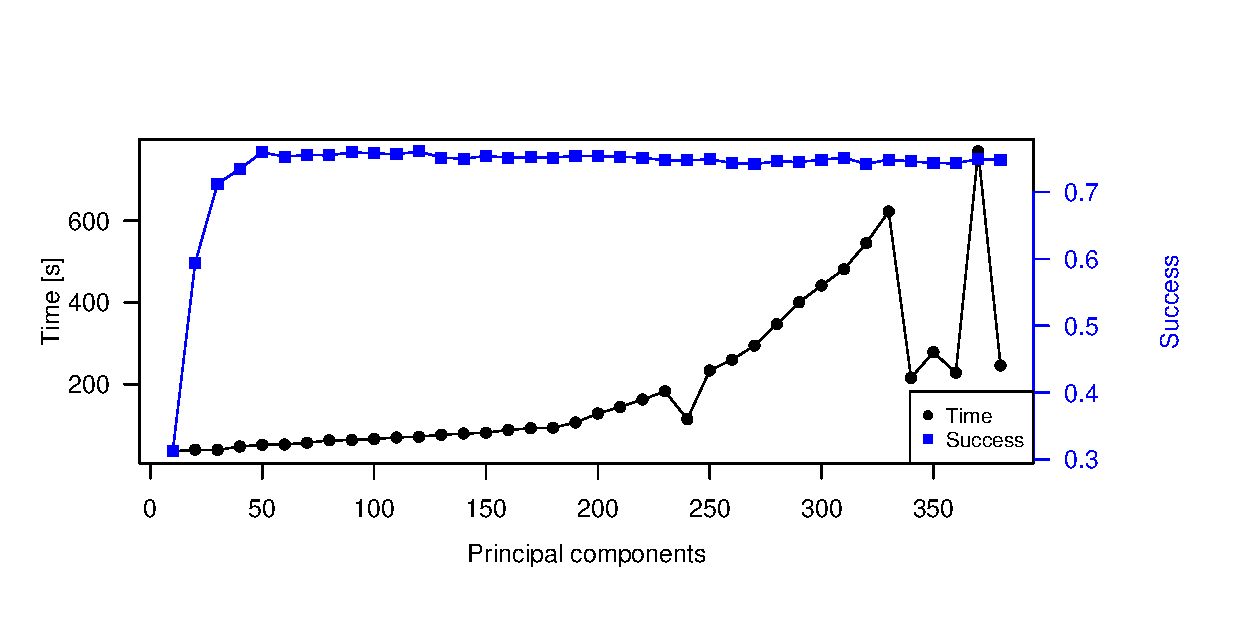
\includegraphics[width =0.8 \textwidth]{graphics/pca_timing}
\caption{Timing of running the PCA with different principle components. 
The data was run on Group 3 member 1's data on 100 DPI. 
The percentage of successful predictions is also measured with the same data.}
\label{fig:pca_timing}
\end{figure}

\begin{figure}
\centering
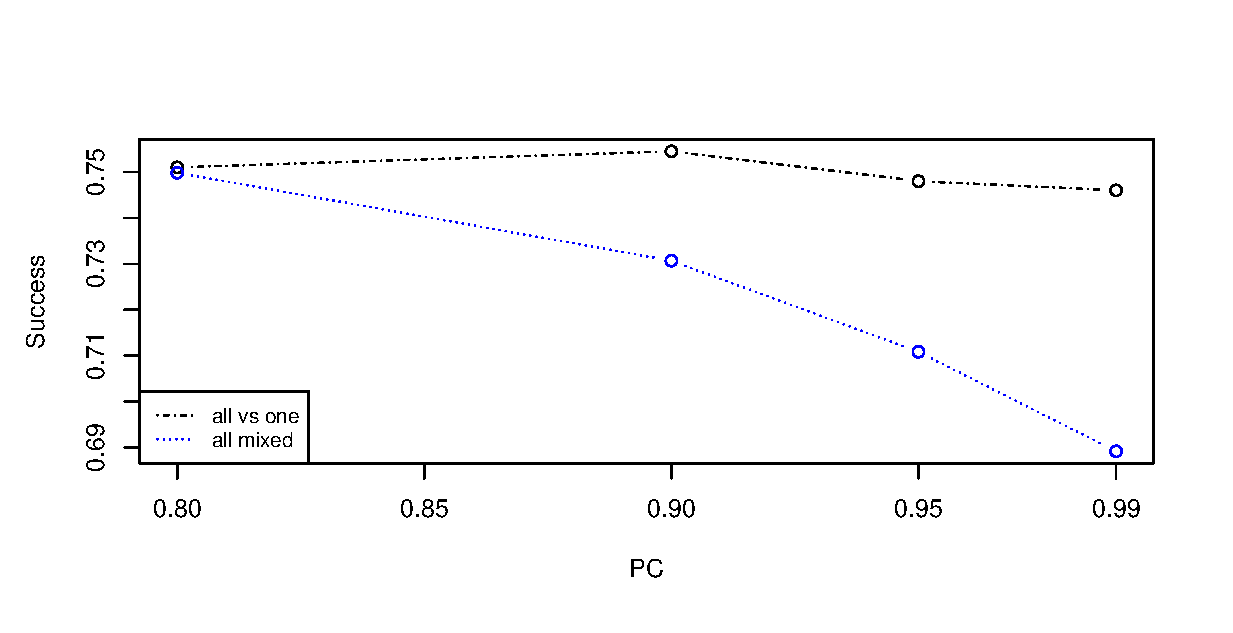
\includegraphics[width =0.8 \textwidth]{graphics/pca_success}
\caption{Percentage of successful predictions with increasing percentage of principle components used.
The data was run on Group 3 member 1's data on 100 DPI. }
\label{fig:pca_success}
\end{figure}

